\documentclass[a4paper,11pt]{article}

%\usepackage{natbib}
\usepackage{amsthm}
\usepackage{amsfonts}
\usepackage{amssymb}
\usepackage{amsmath}
\usepackage{latexsym}
\usepackage{graphicx}
\usepackage{blindtext}

\usepackage{doc}
\renewcommand{\figurename}{Obr.}
\renewcommand{\tablename}{Tab.}

\newtheorem*{theorem}{Theorem}
\theoremstyle{definition}
\newtheorem*{definition}{Definition}

\hoffset -1in \topmargin 0mm \voffset 0mm \headheight 0mm
\headsep0mm
\oddsidemargin  20mm     %   Left margin on odd-numbered pages.
\evensidemargin 20mm     %   Left margin on even-numbered pages.
\textwidth   170mm       %   Width of text line.
\textheight  252mm

\makeatletter
\renewcommand\@openbib@code{%
     \advance\leftmargin  \z@ %\bibindent
      \itemindent \z@
     % Move bibitems close together
     \parsep -0.8ex
     }
\makeatother

\makeatletter
\renewcommand\section{\@startsection {section}{1}{\z@}%
                                   {-3.5ex \@plus -1ex \@minus -.2ex}%
                                   {1.5ex \@plus.2ex}%
                                   {\large\bfseries}}
\makeatother

\makeatletter
\renewcommand\subsection{\@startsection {subsection}{1}{\z@}%
                                   {-3.5ex \@plus -1ex \@minus -.2ex}%
                                   {1.5ex \@plus.2ex}%
                                   {\normalsize\bfseries}}
\makeatother

\makeatletter
	\setlength{\abovecaptionskip}{3pt}   % 0.25cm 
	\setlength{\belowcaptionskip}{3pt}   % 0.25cm 
\makeatother

\begin{document}
\pagestyle{empty}

\begin{center}
{\bf \Large Bin picking}
\end{center}

\smallskip
\begin{center}
{\large Bohumil Velen}
\end{center}

\smallskip
\begin{center}
Faculty of Mechanical Engineering, Brno University of Technology\\
Institute of Automation and Computer Science\\
Technicka 2896/2, Brno 616 69, Czech Republic\\
209493@vutbr.cz\\
\end{center}

\bigskip
\noindent Abstrakt: \textit{Tato seminární práci se zabívá problémem bin picking, kde díly, které vyndáváme z kontejneru jsou chaoticky rozmístěny. O vybrání dílu z kontejneru se stará 3D skener a průmyslový robot. Tato technologie má nahradit stereotipní práci v průmyslu.}

\vspace*{10pt} \noindent Klíčová slova: \textit{Bin picking, 3D skener, stereo kamera, strukturované světlo, laserová triangulce, robotická ramena}

\bigskip
\section{Úvod}
\label{sec:1}
Bin picking je aplikace založena na dvou technologiích: strojové vidění a na práci s robotem. Spojení těchto dvou technologií umožňuje vyndávání dílů, které jsou uspořádáný chaoticky. Díly jsou automaticky vyndávány pomocí robotického ramene, které dostává informace získané ze strojového vidění. Strojové vidění rozpoznává polohu jednotlivých dílů uvnitř kontejneru. Navíc určuje, který díl je nejvhodnější vytáhnout, čímž optimalizuje celý proces. Pozice dílu je určena v 3D prostoru, tudíž jsme schopni robotickým ramenem zachytit díl skoro v každé pozici. \cite{6415038} 
\\
\\Proces bin pickingu má následující kroky:

\begin{itemize}
\item Vyhledání a identifikace dílu v kontejneru. Nalezení polohy a orientace.
\item Rozpoznání vzdálenosti dílu a výpočet optimální trajektorie ve 3D prostoru.
\item Uchopení dílu pomocí chapadla, případně přísavky. 
\item Vyjmutí z kontejneru a umístění na zvolenou polohu.
\end{itemize}

Všechny tyto kroky se provádí autonomně. 
\cite{atria} 

\begin{figure}[h]
\begin{center}
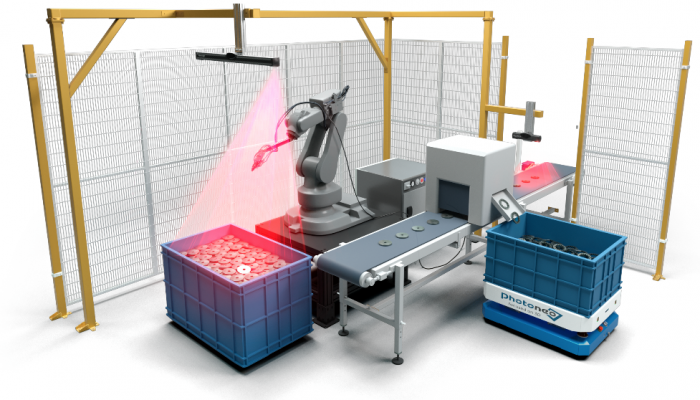
\includegraphics[scale=0.5]{image/binpicking.png}
\caption{Bin picking v praxi \cite{sodavision}}
\label{fig:1}
\end{center}
\end{figure}
\newpage
\section{Popis buňky}
\label{sec:2}
V ideálním případě je robotická buňka umístěna na začátku automatizované montážní linky. To umožňuje optimální tok materiálu a zajišťuje nepřetržité zásobování výroby. Řízení systému komunikuje s PLC a řídí roboty a kamerový systém. V praxi se buňka skládá většinou z 3D skeneru a z průmyslového robota a chapadla (přísavky). 
\begin{figure}[h]
\begin{center}
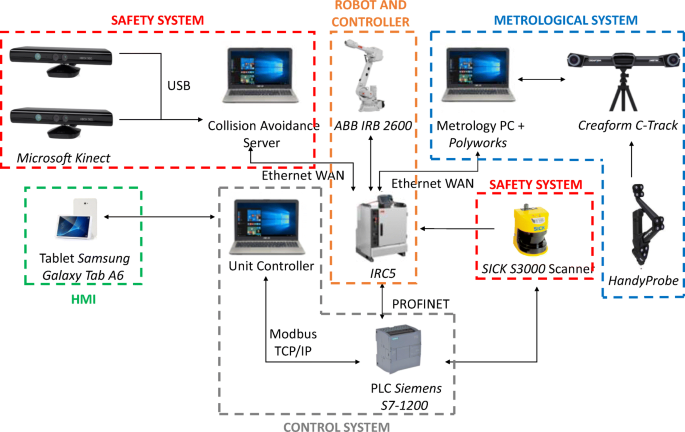
\includegraphics[scale=0.5]{image/descriptionbinpickingcell.png}
\caption{Struktura řídícího systému}
\label{fig:2}
\end{center}
\end{figure}

\section{3D senzor}
\label{sec:3}
Obecným výstupem 3D kamery je obrovské množství bodů. Současné 3D senzory se obvykle dělí do tří základních skupin: stereo kamery, strukturované světlo a laserová triangulace.

\subsection{Stereo kamery}
\label{subsec:1}
Pomocí dvou kamer vedle sebe vytváří stereo vidění prakticky okamžitý odhad vzdáleností prvků ve scéně. Detekce vzdáleností slouží jako primární vodítko pro detekci věcí, které vyčnívají do hloubky z pozadí. Kromě rychlého měření hloubky je stereo vidění vysoce efektivní pro segmentaci objektů a měření jejich velikosti a tvaru. V konečném důsledku stereo vidění zjednodušuje interpretaci dat. \cite{4198262}
\begin{figure}[h]
\begin{center}
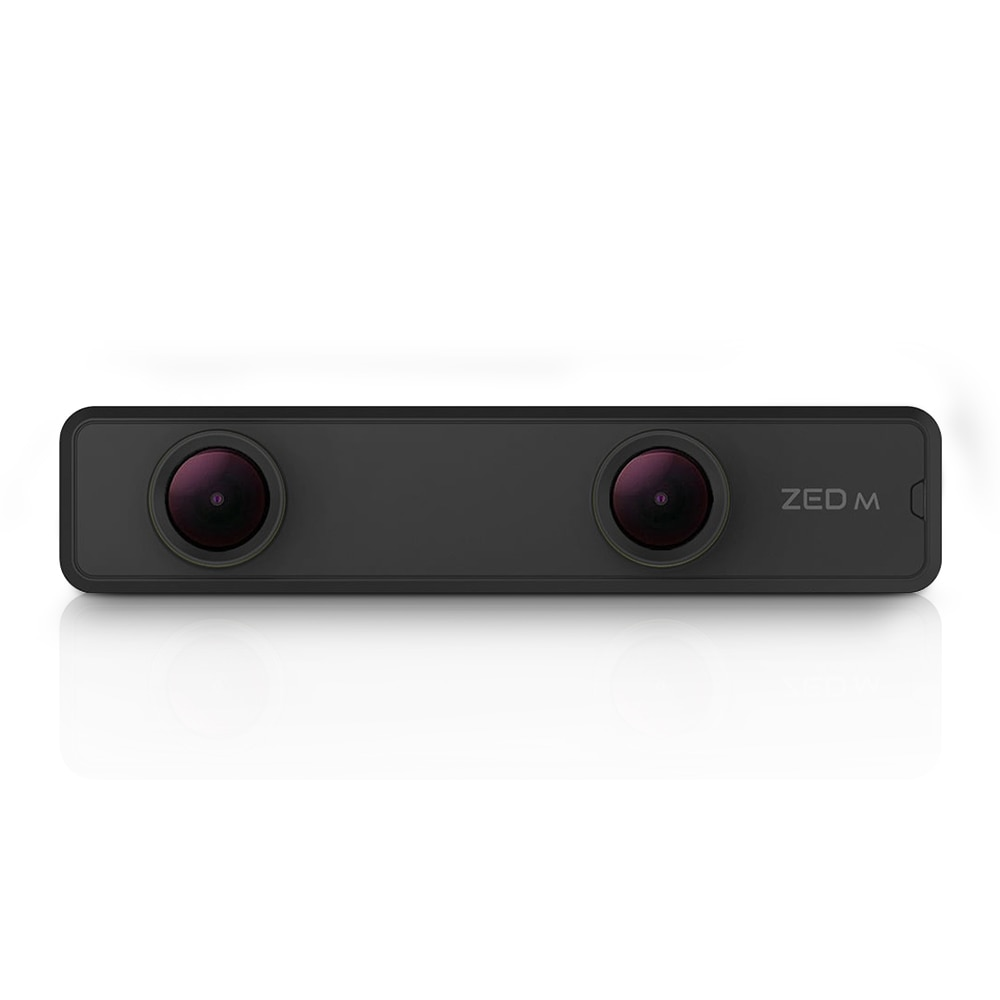
\includegraphics[scale=0.2]{image/stereokamera.jpg}
\caption{Stereo kamera}
\label{fig:2}
\end{center}
\end{figure}

\subsection{Strukturované světlo}
\label{subsec:2}
Základní funkce strukturovaného světelného skeneru je jednoduchá: promítnete strukturovaný světelný vzor na objekt a poté jej natočíte alespoň  jednou kamerou, abyste zachytili způsoby, jakými objekt deformuje světelný vzor.\cite{Geng:11}

\begin{figure}[h]
\begin{center}
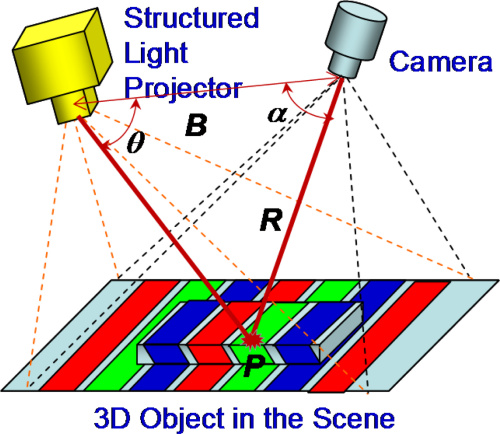
\includegraphics[scale=2.6]{image/getImage.jpg}
\caption{Princip strukturovaného světla \cite{Geng:11}}
\label{fig:3}
\end{center}
\end{figure}

V dřívějších dobách bílé světlo, ale dnes modré světlo promítané ze sofistikovaných LED díky své zvýšené přesnosti a vyšší odolnosti vůči rušivým silám, jako jsou např. odrazy. 


\subsection{Laserová triangulace}
\label{subsec:3}
Laserová triangulace je technika strojového vidění používaná k zachycení 3 rozměrných měření spárováním zdroje laserového osvětlení s kamerou. Laserový paprsek i kamera jsou namířeny na cíl kontroly, avšak použitím známého úhlového posunu ($\alpha$) mezi laserovým zdrojem a snímačem kamery je možné měřit hloubkové rozdíly pomocí trigonometrie. \cite{649437}

\begin{figure}[h]
\begin{center}
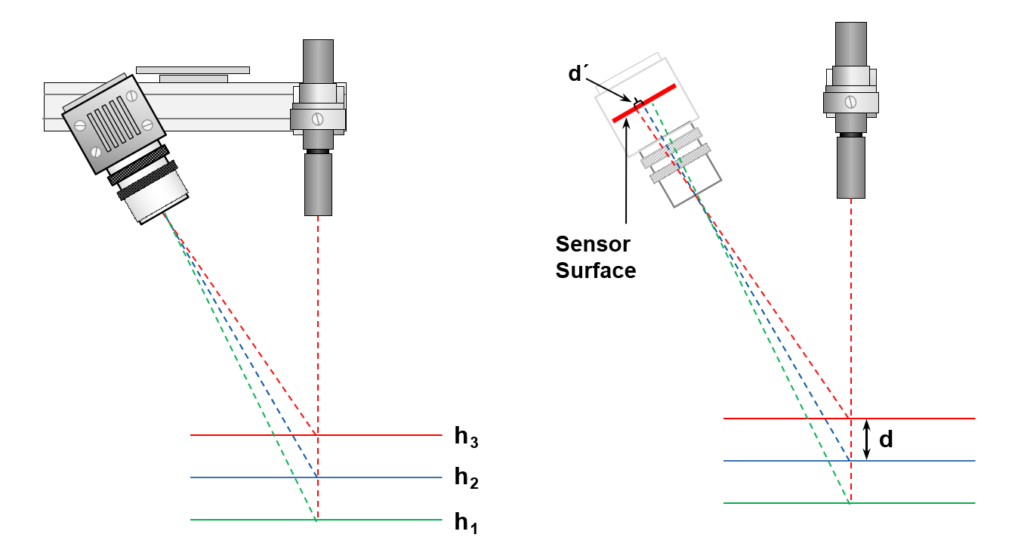
\includegraphics[scale=0.35]{image/lasertriangular.png}
\caption{Princip laserové triangulace \cite{649437}}
\label{fig:4}
\end{center}
\end{figure}

\subsection{Srovnání jednotlivých typu kamer}
\label{subsec              :4}
Srovnání jednotlivých typů 3D skenrů najdeme v tabulce \ref{tab:1}. 
\begin{table}[h] 
\begin{center}
\caption{Porovnání jednotlivých typů 3D senzorů \cite{3Dscener}} 
\label{tab:1}
\begin{tabular}{llll}
\hline\noalign{\smallskip}
  & stereo vidění & strukturované světlo & laserová triangulace\\
\noalign{\smallskip}
\hline\noalign{\smallskip}
Vzálenost & střední & střední & nízká/střední\\
Rozlišení & střední & vysoká  & vysoká\\
Hloubková přesnost & střední & vysoká  & vysoká\\
3D snímací frekvence & vysoká & střední  & nízká\\
Tmavé objekty & nízký & vysoká  & střední\\
Lesklé objekty & nízký & střední  & vysoká\\
Cena & nízký/střední & vysoká  & vysoká\\
\hline
\end{tabular}
\end{center}
\end{table}



\newpage
\section{Průmyslové roboty}
\label{sec:4}
Využití průmyslových robotů zjednodušuje a urychluje práci v mnoha odvětvích, přináší maximální produktivitu a přesnost. Roboti jsou v dnešní době nedílnou součástí zemědělství, stavebnictví, výroby, těžby i lékařství. Podle způsobu použití a konstrukce dělíme průmyslové roboty do několika skupin.
\\ Druhy robotů podle kostrukce:
\begin{itemize}
\item Kartézské roboty
\item SCARA roboty
\item Kloubové roboty
\item Dvouramenné roboty
\item Šestiosé roboty
\item Delta roboty
\end{itemize}
Každý robot má jiné stupně pohybu, proto je vhodný každý na jinou práci. Při využití technologie bin picking se nejvíce využívají šestiosé roboty. 
\\Největšími výrobci průmyslových robotů jsou ABB, Fanuc, KUKA, Yaskawa a další.
\begin{figure}[h]
\begin{center}
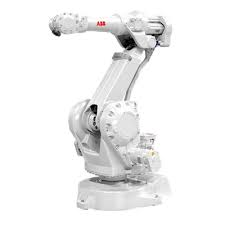
\includegraphics[scale=1.2]{image/robot.jpg}
\caption{Průmyslový robot od firmy ABB}
\label{fig:6}
\end{center}
\end{figure}


\newpage
\section{Závěr}
\label{sec:5}
Tato práce se zabývala bin pickingem a jejími jednotlivými částmi. Jedna z částí bin pickkingu je systém 3D vidění, které umožňuje nalezení, umístění a orientaci dílů v kontejneru. Pro 3D vidění se používají 3D skenery, to můžou být stereo kamery, kamery se strukturovaným světlem a s laserovou triangulací. Další částí je také průmyslový robot. V půmyslu najdeme spousty druhů robotů. Nejčastějsím typem robota používaný v průmyslu je šestiosý robot. Poslední důležitou částí je chapadlo, díky němuž dokážeme vyndávat díly z kontejneru a pokládat je na určenou polohu. Díky této technologii jsme schopni nahradit stereotypní práci, kterou dříve museli vykonávat lidé. 

% References
%
\newpage
\begingroup
\makeatletter
\renewcommand\section{\@startsection {section}{1}{\z@}%
                                   {-3.5ex \@plus -1ex \@minus -.2ex}%
                                   {4.5ex \@plus.2ex}%
                                   {\large\bfseries}}
\makeatother

\renewcommand{\refname}{Seznam literatury}
\bibliography{references}{}
\bibliographystyle{ieeetr}
\endgroup

\end{document}